\documentclass[a4paper]{scrartcl}
\usepackage[utf8]{inputenc}  
\usepackage[T1]{fontenc}
\usepackage{lmodern}           
\usepackage[ngerman]{babel}


%\usepackage[perpage,bottom]{footmisc} % Footnote configuration.

\usepackage{amsmath} % More math.
\usepackage{amssymb} % More symbols.
\usepackage{fancyhdr} % For header and footer format
%\usepackage{fancyref} % For fancy references
\usepackage{listings} % For code listings
\usepackage{booktabs} % For tables
\usepackage[perpage,bottom]{footmisc} % Footnote configuration
\usepackage{graphicx} % For includegraphics
\usepackage[page,titletoc]{appendix} % For appendix in toc
\usepackage{color} % For colors, not sure if I truly need it anymore
\usepackage{caption} % For nicer listing captions
\usepackage{xspace} % For horizontal space.
\usepackage{pst-gantt} % For GANTT chart.
\usepackage{subfigure} % For placing figures next to each other.

% Keine Ahnung warum, aber "`bla"' funktioniert bei mir nicht.
\newcommand{\enquote}[1]{\glqq{}#1\grqq{}}

% Big O
\newcommand{\bigO}{\ensuremath{\mathcal{O}}}

% Hyperref macht Links hinter die Sections und manipuliert PDF-Metadaten:
\usepackage[
colorlinks=false,
pdfborder={0 0 0},
pdftitle={Zufällige Polygone und kürzeste Wege},
pdfsubject={Abschlussbericht zum Softwareprojekt \enquote{Zufällige Polygone und kürzeste Wege}},
pdfauthor={Steve Dierker, Marcel Ehrhardt, Jannis Ihrig, Malte Rohde, Sebastian Thobe, Kadir Tugan}
%pdfkeywords={}
]{hyperref}
\usepackage{breakurl}

% Pimp my listings environment.
% Credits go to stackoverflow:
% http://stackoverflow.com/questions/741985/latex-source-code-listing-like-in-professional-books
\lstset{
         basicstyle=\footnotesize\ttfamily, % Standardschrift
         numberstyle=\tiny,          % Stil der Zeilennummern
         numbers=left,
         stepnumber=1,
         numbersep=7pt,              % Abstand der Nummern zum Text
         keywordstyle=\bfseries\ttfamily,
         tabsize=2,                  % Groesse von Tabs
         extendedchars=true,         %
         breaklines=true,            % Zeilen werden Umgebrochen       
         showspaces=false,           % Leerzeichen anzeigen ?
         showtabs=false,             % Tabs anzeigen ?
         %frame=b,                   % Linie unten
         breakatwhitespace=true,
         xleftmargin=17pt,
         framexleftmargin=17pt,
         framexrightmargin=5pt,
         framexbottommargin=4pt,
         showstringspaces=false      % Leerzeichen in Strings anzeigen ?      
 }

% Pimp my captions.
\DeclareCaptionFont{white}{\color{white}}
\DeclareCaptionFormat{listing}{\colorbox[cmyk]{0.43, 0.35, 0.35,0.01}{\parbox{\textwidth}{\hspace{15pt}#1#2#3}}}
\captionsetup[lstlisting]{format=listing,labelfont=white,textfont=white, singlelinecheck=false, margin=0pt, font={bf}}

% Listing environment for C
\lstnewenvironment{code}[1][]
  {\noindent\minipage{\linewidth} 
   \lstset{language=C,#1}}
  {\endminipage}

% Konfiguration der Titelseite:
\title{
{\normalsize Softwareprojekt über Anwendung effizienter Algorithmen\\ Wintersemester 2011/12}
\\[4ex] 
{\Large Abschlussbericht zum Softwareprojekt\\ \enquote{Zufällige Polygone und kürzeste Wege}}
\\[6ex]
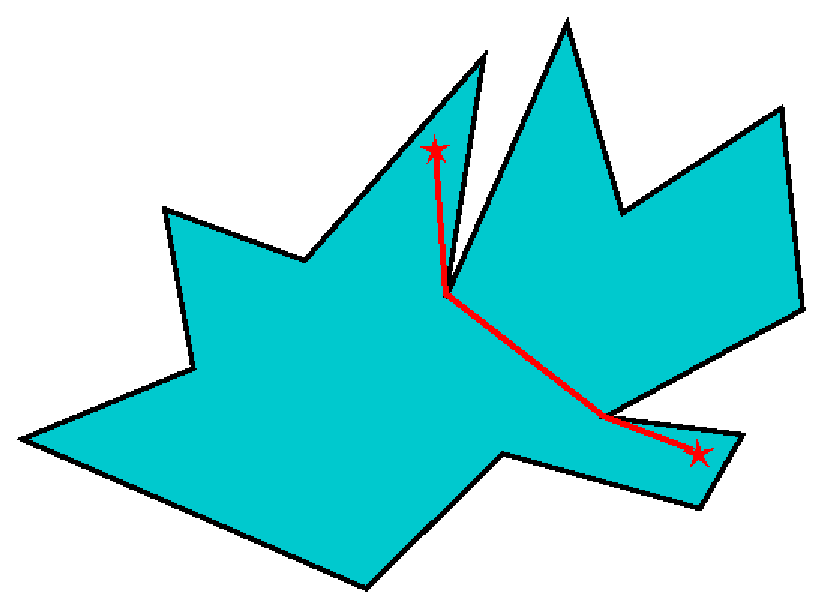
\includegraphics[width=0.4\textwidth]{img/polygons}
\\[3.5cm]}
\author{Steve Dierker \and Marcel Ehrhardt \and Jannis Ihrig \and Malte Rohde \and Sebastian Thobe \and Kadir Tugan}

\date{\vspace{2.5cm} \today{}}

\begin{document}

\begin{titlepage}
\pagenumbering{alph}
\maketitle
\thispagestyle{empty}
\vfill{}
\end{titlepage}

\pagestyle{empty}
\pagenumbering{roman}
%\include{parts/abstract}
\tableofcontents
\clearpage

\pagenumbering{arabic}
\pagestyle{fancy}
\lhead[]{}
\rhead[\nouppercase{\rightmark}]{\nouppercase{\rightmark}}
\setcounter{page}{1}

% Hier hin unsere Kapitel.
\section{Einleitung}

  Die algorithmische Geometrie als Teilgebiet der Informatik beschäftigt sich
  mit der algorithmischen Lösung geometrischer Probleme. Einfache Polygone
  (überschneidungsfreie, zusammenhängende, planare Vielecke) bilden die
  Grundlage vieler Aufgabengebiete der algorithmischen Geometrie. Als
  naheliegendes Beispiel bezeichnet die Triangulierung die Zerlegung eines
  Polygons in eine Menge von Dreiecken, die die Fläche des Polygons
  überdecken. Diese Dreieckszerlegung ermöglicht die Lösung einer ganzen Reihe
  weiterer geometrische Probleme.

  Zum Testen und zur Evaluation polygon-basierter geometrischer
  Algorithmen ist es oft von Vorteil, über eine beliebige Menge einfacher
  Polygone zu verfügen, wobei diese, um eine gewisse Aussagekraft der
  Experimente zu gewährleisten, möglichst alle (in einem
  definierten planaren Raum) vorstellbaren Polygone erzeugen können sollten. Die
  massenweise Erzeugung solcher \emph{zufälliger Polygone} ist ein
  Forschungsgebiet, dem in den vergangenen Jahrzehnten daher vermehrt
  wissenschaftliche Aufmerksamkeit zugekommen ist. Die entstandenen
  Lösungswege und Algorithmen unterscheiden sich unter anderem in ihrer
  Komplexität, im Speicherverbrauch sowie in der Art und
  \enquote{Zufälligkeit} der erzeugten Polygone.

  Der vorliegende Text ist der Abschlussbericht des Softwareprojekts
  \emph{Zufällige Polygone und kürzeste Wege}, welches im Rahmen des Moduls
  \enquote{Softwareprojekt: Anwendung von Algorithmen} unter Leitung von Prof.
  Dr. Günter Rote durchgeführt wurde. Das Ziel des Projekts war die
  Entwicklung einer Softwarebibliothek, welche über verschiedenene Algorithmen
  zur Erzeugung zufälliger Polygone verfügen und diese unter anderem
  über eine grafische Schnittstelle dem Benutzer zur Verfügung stellen sollte.
  Das Projekt wurde mit Ende des Wintersemesters 2011/2012 abgeschlossen.

  Im Folgenden werden wir zunächst die Zielsetzung des Projekts, funktionale
  und nicht-funktionale Anforderungen an die zu implementierende Software,
  sowie Einschränkungen der Zielsetzung darstellen. Anschließend erfolgt eine
  kurze Erläuterung des von uns gewählten Entwicklungsprozesses und dessen
  Umsetzung. Im Hauptteil des Berichts gehen wir detailliert auf die
  Eigenschaften der einzelnen Algorithmen sowie auf die während der
  Entwicklung aufgetretenden Probleme und deren Lösungen ein. In
  Kapitel~\ref{sec:manual} findet der Leser einen umfassenden
  \emph{Benutzerleitfaden} für die entstandene Softwarelösung. Im letzten
  Kapitel schließen wir den Bericht mit einem kurzen Fazit zum Projektablauf
  sowie zu unserer Einschätzung der Brauchbarkeit der Software.

\section{Projektstruktur}

  Das Projekt \emph{Zufällige Polygone} wurde im Wintersemester 2011/2012 in
  einem Zeitraum von rund 4 Monaten durchgeführt. Im Folgenden werden wir
  zunächst die Ziele des Projekts darstellen, den zeitlichen Ablauf darlegen
  und abschließend den gewählten Entwicklungsprozess beschreiben.

  \subsection{Zielsetzung \& Einschränkungen}

    Das Hauptziel des Projekts war die Implementierung einer Reihe von
    Algorithmen, die der Erzeugung zufälliger einfacher Polygone dienen. Vom
    verantwortlichen Dozenten wurden dabei vier wissenschaftliche Artikel zur
    Verfügung gestellt, in denen insgesamt 7 derartige Algorithmen beschrieben
    werden. Darüberhinaus sollte ein vom Dozenten mitentwickelter \emph
    {Shortest-Path}-Algorithmus~\cite{asano11shortestpath} implementiert werden,
    welcher in einem gegebenen Polygon die kürzeste Verbindung zwischen zwei
    gewählten Punkten errechnet. Folgende weitergehenden Anforderungen an die zu
    entwickelnde Software waren gegeben:

    \begin{itemize}
      \item Massenweise (\emph{batch}) Erzeugung von zufälligen Polygonen 
            per Kommandozeile
      \item Export eines oder vieler Polygone als CSV-Datei 
            (\emph{comma-separated value})
      \item Grafische Oberfläche
      \begin{itemize}
        \item Auswahl und Konfiguration des Algorithmus
        \item Visualisierung der Funktionsweise des Algorithmus
        \item Auswahl der Punkte für den Shortest-Path-Algorithmus
        \item Visualisierung der Funktionsweise des Shortest-Path-Algorithmus
      \end{itemize}
      \item Statistische Analyse der Algorithmen hinsichtlich ihrer Laufzeit 
            und den Eigenschaften der erzeugten Polygone
    \end{itemize}

    Als Programmiersprache wählten wir \emph{Java}, da alle Projektmitglieder
    über Erfahrung in der Java-Programmierung verfügten und die Sprache sowohl
    die gewünschte Performanz als auch eine ausreichend umfangreiche
    Standardbibliothek bot. Aufgrund des begrenzten zeitlichen Rahmens des
    Projekts mussten jedoch einige Einschränkungen in Bezug auf die
    mathematische Korrektheit der entwickelten Software getroffen werden.
    Zunächst ist hier die Entscheidung für die Verwendung von Gleitkomma- und
    gegen die (ausschließliche) Verwendung von Ganzzahlen zu nennen. Zwar
    ermöglichen Gleitkommazahlen die einfache und CPU-gestützte
    Divisionsoperation, jedoch kann es durch die begrenzte Auflösung der
    Gleitkommazahlen (bspw. 64 Bit bei Variablen des Typs \emph{double}) zu
    Rundungsungenauigkeiten kommen.

    Eine weitere, mithin gravierendere Einschränkung ist der Verzicht auf einen
    \emph{General Position}-Test (im Deutschen manchmal \enquote{allgemeine
    Lage}) vor Ausführung der Algorithmen. Eine Menge von Punkten in der Ebene
    befindet sich in \emph{general position}, wenn

    \begin{enumerate}
      \item keine zwei Punkte identisch sind,
      \item keine drei Punkte auf einer Geraden liegen und
      \item keine 4 Punkte auf einem Kreis liegen.
    \end{enumerate}

    Manche Polygon-Algorithmen versagen, wenn eine dieser Eigenschaften,
    insbesondere 2., für die gegebene Punktmenge nicht erfüllt ist. Zwar lässt
    sich eine Punktmenge leicht auf GP überprüfen, jedoch ist dieser Test vor
    allem für große Punktmengen sehr rechenintensiv. Der von uns vorübergehend
    verwendete naive Algorithmus zum GP-Test wies ein asymptotisches Wachstum
    von $\bigO\left(n^3\right)$ auf, sodass die Laufzeit des GP-Tests bisweilen
    die Laufzeit des Algorithmus weit übertraf. Als Konsequenz hieraus
    verzichteten wir auf einen GP-Test, sodass eine nicht in GP befindlichen
    Punktmenge zu undefinierte Ergebnissen des Programms führen kann. Mit der
    Verwendung von 64-bit \emph{double}-Variablen zur Darstellung der $x$- und
    $y$-Koordinaten ist eine solche Situation jedoch äußerst unwahrscheinlich.

  \subsection{Zeitplan}

    Wir präsentieren hier den Zeitplan des Projekts in Form eines GANTT-
    Diagramms, welches auch während der Projektarbeit Verwendung fand. Da das
    Diagramm laufend an den aktuellen Entwicklungsstand angepasst wurde,
    entspricht es nun nahezu exakt dem tatsächlichen zeitlichen Ablauf der
    Entwicklung.

    \begin{figure}[h]
    \begin{center}
    \bfseries\fontsize{5}{5}\selectfont
    \newpsstyle{TaskStyleA}{fillstyle=solid,fillcolor=red}
    \begin{PstGanttChart}[% 
        yunit=1.0,
        xunit=0.68,
        ChartUnitIntervalName=KW,
        ChartUnitBasicIntervalName=KW,
    %    ChartModulo,
        ChartModuloValue=52,
        TaskUnitIntervalValue=14,
        TaskUnitType=KW,
        ChartStartInterval=43,
        ChartShowIntervals]{15}{15}
    \psset{TaskStyle=TaskStyleA}
    \PstGanttTask[TaskInsideLabel={PolygonGenerator interface}]{0}{4}
    \PstGanttTask[TaskInsideLabel={Data structures scratch}]{0}{4}
    \PstGanttTask[TaskInsideLabel={GUI scratch}]{0}{4}
    \PstGanttTask[TaskInsideLabel={Data structures done}]{1}{3}
    \PstGanttTask[TaskInsideLabel={First polygon algorithms}]{1}{4}
    \PstGanttTask[TaskInsideLabel={ShortestPathGenerator interface}]{1}{4}
    \PstGanttTask[TaskInsideLabel={All polygon algorithms}]{3}{4}
    \PstGanttTask[TaskInsideLabel={Shortest path algorithm}]{3}{4}
    \PstGanttTask[TaskInsideLabel={GUI}]{3}{4}
    \PstGanttTask[TaskInsideLabel={History data structure}]{6}{4}
    \PstGanttTask[TaskInsideLabel={Step-by-step visualisation}]{6}{4}
    \PstGanttTask[TaskInsideLabel={Statistics backend}]{6}{4}
    \PstGanttTask[TaskInsideLabel={Improved GUI}]{10}{3}
    \PstGanttTask[TaskInsideLabel={Statistics visualisation}]{10}{3}
    \PstGanttTask[TaskInsideLabel={Cleanup for release}]{12}{3}
    \end{PstGanttChart}
    \end{center}
    \label{fig:gantt}
    \end{figure}

  \subsection{Entwicklungsprozess}

    Der von uns gewählte Entwicklungsprozess folgte keinem fest definierten
    Modell (bspw. SCRUM), beinhaltete jedoch einige prozessunterstützende
    Maßnahmen, die vor allem der kontinuierlichen Kommunikation innerhalb des
    Teams dienen sollten. Die folgenden Prozesselemente stellten sich als
    hilfreich heraus und wurden während der Projektarbeit konsequent
    beibehalten:

    \begin{itemize}
      \item Iterative Herangehensweise, stets lauffähige Version im Repository.
      \item Wöchentliche Team-Meetings zur Besprechung des aktuellen Stands, 
            der in der vergangenen Woche erledigten Arbeit sowie der für die 
            folgende Woche geplanten Arbeitspakete. Schriftliche Protokolle 
            dienten der Information abwesender Teammitglieder.
      \item Arbeitspakete werden stets in 2er-Teams bearbeitet, 
            unter anderem um den Busfaktor\footnote{\url{http://en.wikipedia.org/wiki/Bus_factor}} zu erhöhen.
      \item Unregelmäßig stattfindende \emph{coding sessions}.
    \end{itemize}

    Insbesondere der letztgenannte Punkt entwickelte sich im Laufe des Projekts
    zu einer wichtigen Maßnahme, um sowohl Verzögerungen im Zeitplan gering zu
    halten, als auch das Wissen über den geschriebenen Code möglichst
    gleichmäßig auf die Teammitglieder zu verteilen. Die \emph{coding sessions}
    wurden von allen Teammitgliedern als überaus produktiv empfunden, oftmals
    konnten an einem Tag eine ganze Reihe Arbeitspakete abgeschlossen werden.
    Zudem zeigten sich Fehler im Code oft erst, während mehrere, vorher
    unbeteiligte Teammitglieder den Code der anderen ausgiebig testeten.

    Entscheidungen im Team wurden weitestgehend per Konsens geschlossen. Für den
    seltenen Fall einer Unstimmigkeit wurde zuvor Jannis Ihrig zum Projektleiter
    bestimmt. Der Projektleiter vertrat das Projekt zudem als Ansprechpartner
    gegenüber dem Dozenten.

\section{Algorithmen zur Polygongenerierung}

  In Tabelle~\ref{algo_table} findet sich eine Auflistung der in der
  entstandenen Softwarelösung implementierten Algorithmen. Die meisten dieser
  Algorithmen bedürfen einer vorgegebenen Punktmenge, aus welcher ein simples
  Polygon konstruiert wird. Der \enquote{Random Polygon Algorithm} hingegen
  erhält als initialie Punktmenge lediglich die Eckpunkte eines Dreiecks und
  erzeugt im gegebenen begrenzten Raum eine konfigurierbare Anzahl weiterer
  Punkte. Der Algorithmus von Virmani verändert als einziger Algorithmus die
  Position der Punkte der vorgegebenen Punktmenge.

  Die in Tabelle~\ref{algo_table} angegebene \enquote{Laufzeit} bezeichnet die
  theoretisch kleinste obere Schranke für das asymptotische Wachstum der
  Laufzeitsfunktion der Algorithmen, in Abhängigkeit der Anzahl der Punkte $n$.
  In einigen Fällen lässt sich diese jedoch nicht bestimmen, bzw. beschreibt
  eine erwartete Laufzeit bei randomisierten Algorithmen (bspw. Permute \&
  Reject). Da die Laufzeit einiger Hilfsfunktionen (z.B. Polygon-Gerade-
  Schnittberechnung) in unserer Implementierung nicht ideal ist, weicht die
  Laufzeit der Algorithmen in der Implementierung zum Teil von der erwarteten
  Laufzeit ab.

  \begin{table}[ht]
    \begin{center}
    \caption{Polygon-Algorithmen}
    \begin{tabular}{lcc} 
      \toprule
      Algorithmus & erw. Laufzeit & Laufzeit (Impl.) \\
      \midrule
      Permute \& Reject & $\bigO(n!)$ & $\bigO(n!)$ \\
      Incremental Construction \& Backtracking & $\bigO(n!)$ & $\bigO(n!)$ \\
      Space Partitioning & $\bigO(n^2)$ & $\bigO(n^2)$\\
      Steady Growth & $\bigO(n^2)$ & ... \\
      2-Opt Moves & $\bigO(n^3)$ & $\bigO(n^4)$ \\
      Velocity Virmani & ... & ...\\
      Two Peasants & $\bigO(n \log n)$ & $\bigO(n \log n)$ \\
      Random Polygon Algorithm & $\bigO(n^2 \log n)$ & ... \\
      \bottomrule
    \end{tabular}
    \label{algo_table}
    \end{center}
  \end{table}

  Im Folgenden wird die Funktionsweise der einzelnen Algorithmen erläutert und
  auch besondere Eigenschaften der erzeugten Polygone dargestellt.

\subsection{Permute \& Reject}

\begin{figure}[h]
\begin{center}

\includegraphics[width=0.3\textwidth]{img/permute16.eps}
\end{center}
\caption{Polygon mit 16 Punkten (Permute \& Reject)}
\label{fig:permute16}
\end{figure}

\emph{Permute \& Reject} ist der einfachste in der Software enthaltenene Algorithmus zur Erzeugung von simplen Polygonen, implementiert nach einer Beschreibung von Martin Held in~\cite{held98polygons}.
\subsubsection{Algorithmus}
Der Algorithmus basiert auf der zufälligen Erzeugung von $n$ Kanten zwischen $n$ gegebenen Punkten, sodass von jedem Punkt zwei Kanten ausgehen. Anschließend wird überprüft, ob das entstandene Polygon \enquote{simpel}, d.h. überschneidungsfrei ist. Falls nicht, wird das Polygon verworfen und von vorne begonnen.

\begin{code}[caption={Permute \& Reject},label=permutelisting,mathescape=true]
retry:
$P$ $\leftarrow$ given set of points
$p$ $\leftarrow$ remove random point from $P$
while ($P$ not empty)
  $q$ $\leftarrow$ remove random point from $P$
  draw edge from $p$ to $q$
  $p$ $\leftarrow$ $q$
if resulting polygon is NOT simple
  goto retry
\end{code}

\subsubsection{Eigenschaften}
Ausgehend von einer beliebigen Punktmenge kann Permute \& Reject sämtliche möglichen Polygone erzeugen. Jedoch lässt die enorme Laufzeit des Algorithmus eine praktische Verwendung für Polygone mit vielen Punkten nicht zu. Eine -- wenn auch nicht scharfe -- obere Schranke für die Laufzeit lässt sich mit $\bigO(n!)$ beziffern, entsprechend dem Durchprobieren jeglicher möglichen Kombination von Punkten. In unseren Experimenten konnten wir kein Polygon mit mehr als 28 Punkten erzeugen.
\subsection{Incremental Construction \& Backtracking}

\begin{figure}[h]
\begin{center}

\includegraphics[width=0.3\textwidth]{img/icb14.eps}
\end{center}
\caption{Polygon mit 14 Punkten (IC\&B)}
\label{fig:icb14}
\end{figure}

\emph{Incremental Construction \& Backtracking} (IC\&B) ist ein rekursiver Algorithmus zur Erzeugung von simplen Polygonen, implementiert nach einer Beschreibung von Martin Held in~\cite{held98polygons}. 
\subsubsection{Algorithmus}
Die Funktionsweise des Algorithmus ist verhältnismäßig komplex. Ausgehend von einem zufällig gewählten Startpunkt werden rekursiv alle Punkte der gegebenen Punktmenge zur Polygonkette hinzufügt. Zugleich wird in einer speziellen Datenstruktur aufgezeichnet, welche Verbindungen zwischen Punkten aufgrund der zuletzt hinzugefügten Kante des Polygons im weiteren Verlauf des Algorithmus nicht mehr gewählt werden können. Nach dem Hinzufügen eines Punktes zur Polygonkette wird überprüft, ob mit den verbleibenden Punkten ein simples Polygon konstruiert werden kann. Hierzu definiert Held in~\cite{held98polygons} drei Bedingungen, die einzeln und in Reihenfolge auf ihren Wahrheitswert getestet werden. Sollte eine der Bedingungen nicht zutreffen, wird der zuletzt hinzugefügte Punkt wieder entfernt und mit dem nächsten Punkt fortgefahren. Sind ausgehend von einer bestimmten partiellen Polygonkette alle verbleibenden Punkte auf ihre Tauglichkeit als folgender Punkt mit negativem Resultat getestet worden, muss ein weiterer Schritt zurückgegangen werden (\emph{Backtracking}), d.h. ein weiterer Punkt aus der Polygonkette entfernt werden. Für eine weiterführende Erklärung des Algorithmus, siehe~\cite{held98polygons}.

\subsubsection{Eigenschaften \& Implementierungsdetails}
Obgleich die Anzahl der Backtracking-Schritte durch die Verwendung der Kantenmenge auf ein Minimum beschränkt wird, kann es oftmals vorkommen, dass bereits in den ersten Rekursionsschritten des Algorithmus eine \enquote{ungünstige} Kante hinzugefügt wird. In solchen Fällen erfolgen häufig zunächst eine große Anzahl an Rekursions- und Backtrackingschritten, ehe die \enquote{ungünstige} Kante wieder aus der Polygonkette entfernt wird. Dies führt in Verbindung mit der rechenintensiven Pflege der Kantenmenge zu einer schnell wachsenden Laufzeit des Algorithmus. Im (theoretischen) \emph{worst-case scenario} würden $n!$ Schritt benötigt, entsprechend dem Ausprobieren jeder möglichen Permutation der Punktmenge. In der Praxis war es uns nicht möglich, Polygone mit mehr als 20 Punkten zu erzeugen.

Zusätzlich zur für den praktischen Einsatz ungeeignet hohen Laufzeit ist auch der Implementierungsaufwand des Algorithmus nicht zu unterschätzen. Vor allem die Pflege der Kantenmenge im Verlauf der Rekursion und des Backtracking ist durchaus komplex, sodass wir uns in der Implementierung der Einfachheit halber dafür entschieden, in jedem Rekursionsschritt eine Kopie der Kantenmenge anzulegen. Da der Speicherbedarf für die Kantenmenge zumindest quadratisch von der Anzahl der Punkte abhängt, steigt durch diese das asymptotische Wachstum des Speicherbedarfs des Algorithmus auf $\bigO(n^3)$. Aufgrund der geringen möglichen Punktanzahl fällt dieser Speicherbedarf jedoch nicht ins Gewicht.

\subsection{Space Partitioning}

  \begin{figure}[h]
    \begin{center}
      
\includegraphics[width=0.3\textwidth]{img/spacepart200.eps}
    \end{center}
    \caption{Polygon mit 200 Punkten (Space Partitioning)}
    \label{fig:space200}
  \end{figure}

  \enquote{Space Partitioning} ist einer der von T. Auer und M. Held 
  in~\cite{held98polygons} beschriebenen Algorithmen zur Generierung von
  einfachen Polygonen.


  Es handelt sich dabei um einen Divide und Conquer Algorithmus, der, wie der
  Name schon suggeriert, im Divide-Schritt eine vorgegebene Punktmenge in
  Partitionen mittels einem Halbebenenschnitts aufteilt, dann rekursiv Polygone
  in diesen Halbebenen erzeugt und im Merge-Schritt diese Polygone in ein
  einfaches gesamt Polygon zusammensetzt.

  \subsubsection{Algorithmus}

    Wie oben schon beschrieben ist \enquote{Space Partitioning} ein 
    Divide \& Conquer
    Algorithmus, der in der Betrachtung und Umsetzung die Allgemeine Lage
    voraussetzt. \\

    \noindent
    Space Partitioning besteht im wesentlichen aus drei Schritten:
    \begin{itemize}
      \item[1.] Die Berechnung einer Geraden $l$, die den Rand der Halbebenen 
            repr"asentiert und somit die Punktmenge in zwei eindeutige 
            Partitionen teilt
      \item[2.] Die rekursive Konstruktion eines linken und rechten 
            Teilpolygons innerhalb der Partitionen
      \item[3.] Die Zusammenf"ugung dieser Teilpolygone zu einem gesamten 
            Polygon
    \end{itemize}

    \noindent
    Bevor die Rekursion im Space Partitioning Algorithmus ausgef"uhrt werden
    kann, muss diese gesondert initialisert werden, in dem wir einmalig zwei
    Punkte aus der Punktmenge zuf"allig ausw"ahlen und die Partition anhand der
    Geraden, die durch diese zwei gew"ahlten Punkte verl"auft, vornehmen. \\
    Der eigentliche Rekursionsschritt braucht dabei diese Anfangs- und
    Endpunkte, um eine neue Partitionsgerade zu konstruieren. \\
    In der Implementierung wurde darauf geachtet, dass die in der Rekursion
    erstellten Teilpolygone die Anfangs- bzw. Endpunkte an erster bzw. letzter
    Position in dem  Polygonzug zu stehen haben - je nachdem, ob es sich um das
    linke oder rechte Teilpolygon handelt -, wodurch der Merge-Schritt nur an
    den Grenzen der Polylines Duplikate entfernen musste, um das Polygon zu
    erstellen. Au"serdem wurde auf eine CCW-Sortierung der Punkte geachtet.

    % Einbauen?
    %Wir k"onnen insgesamt folgende Beobachtung in einer Invariante ausdr"ucken:
    %Der Schnitt der beiden Teilpolygone besitzt nur eine gemeinsame Kante und diese ist genau
    %die Strecke den gegebenen Anfangs- und Endpunkte.

    % TODO:
    % die im Prozess der Konstruktion im Allgemeinen nicht einfach bleiben

\begin{code}[caption={Space Partitioning}, mathescape=true]
choose two random points $s_f$ and $s_l$ and remove them

left, right $\leftarrow$ partition points in the left/right side of the line $l(s_f, s_l)$

leftPolygon $\leftarrow$ Space Partitioning(left, $s_f$, $s_l$)
leftPolygon $\leftarrow$ Space Partitioning(right, $s_f$, $s_l$)

polygon $\leftarrow$ merge(leftPolygon, rightPolygon)
\end{code}

    \noindent

    Der Rekursionsschritt l"auft analog zum Initialierungsschritt ab. Nur das
    hier die Partitionierung mithilfe der Geraden $l$ (siehe Z.
    \ref{lst:space_line}) erfolgt. Diese Gerade $l$ wird durch einen zuf"allig
    gew"ahlten Anfangspunkt auf der Strecke $s_f$, $s_l$ und einem zuf"alligen
    Endpunkt aus der Punktmenge ``points'' definiert.

\begin{code}[caption={Rekursion Space Partitioning}, 
            mathescape=true, escapeinside={@}{@}]
Space Partitioning(points, $s_f$, $s_l$)

  if points only contains $s_f$ and $s_l$
    return line segment $s_f$, $s_l$

  $s$ $\leftarrow$ choose random and remove point in points
  @\label{lst:space_line}@$l$ $\leftarrow$ choose random line through $s$, which intersects the line segment $s_f$, $s_l$

  left, right $\leftarrow$ partition points in the left/right side of the line $l$

  leftPolygon $\leftarrow$ Space Partitioning(left, $s_f$, $s$)
  rightPolygon $\leftarrow$ Space Partitioning(right, $s$, $s_l$)

  polygon $\leftarrow$ merge(leftPolygon, rightPolygon)

  return polygon
\end{code}

  \subsubsection{Laufzeit}

    Die Laufzeitanalyse von \enquote{Space Partitioning} ist analog zur
    Laufzeitanalyse von Quicksort. Sei $n$ die Anzahl der vorgegebenen
    Punktmenge. Nach der Rekursionsbaum Analysemethode werden in jeder
    Rekursionsebene  h"ochstens $\bigO(n)$ Operationen ausgef"uhrt (Die
    Punktmenge wird komplett unter den Rekursionaufrufen einer Rekursionsebene
    aufgeteilt). Wodurch die Laufzeit sich nur nach der Rekursionstiefe richtet.
    Bei halbwegs gleicher Aufteilung der Partitionen sind nur $\bigO(\log n)$
    Rekursionsebenen, im worst-case $\bigO(n)$ hingegen n"otig.
    \\ Damit hat \enquote{Space Partitioning} eine worst-case Laufzeit von
    $\bigO(n^2)$, aber in vielen F"allen eine sehr viele bessere $\bigO(n \log
    n)$ Laufzeit.

  \subsubsection{Eigenschaften}

    Aufgrund des einfachen Divide \& Conquer Ansatzes und ausschlie"slichen
    Verwendung von Basis-Operationen, wie z.B. eines Orientierungstests, ist
    \enquote{Space Partitioning} der schnellste implementierte Algorithmus dieses
    Projekts. Wodurch \enquote{Space Partitioning} sich f"ur Testpolygone mit gro"sen
    Punktmengen (100.000 Punkte in weniger als 10s) anbietet. Leider ist ``Space
    Partitioning'' nach T.Auer und M. Held~\cite{held98polygons} nicht
    inclusive,  dennoch geben sie in ihrem Paper an, dass bei 100.000
    Durchl"aufen mit 10 Punkten ungef"ahr 10-20\% der generierten Polygone
    Duplikate von bereits generierten waren. Bei 100 Punkten und 100.000
    Durchl"aufen wurde kein Polygon mehrfach erzeugt. Wodurch es, nach ihrere
    Einsch"atzung, bei gro"sen Punktmengen unwahrscheinlich ist, dass Polygone
    mehrfach generiert werden. Au"serdem konnten sie bei ihrerer Datenanalyse
    feststellen, dass man nicht erwarten sollte, dass die erzeugten Polygone
    gleichverteilt auftreten.



\subsection{Steady Growth}

  \begin{figure}[h]
    \begin{center}
      
\includegraphics[width=0.3\textwidth]{img/steady200.eps}
    \end{center}
    \caption{Polygon mit 200 Punkten (Steady Growth)}
    \label{fig:steady200}
  \end{figure}

  \enquote{Steady Growth} ist einer der mehreren im Paper~\cite{held98polygons}
  beschriebenen Algorithmen zur Generierung von einfachen Polygonen.

  \enquote{Steady Growth} konstruiert ein einfaches Polygon, indem er in jeder
  Iteration einen neuen Punkt zu dem Polygon hinzuf"ugt, wobei der Punkt mit
  bestimmten Einschr"ankungen gew"ahlt werden muss, sodass das Polygon in jeder
  Iteration einfach bleibt.

  \subsubsection{Algorithmus}

\begin{code}[caption={Steady Growth}, mathescape=true]
$P_0$ $\leftarrow$ choose random triangle such that no remaining points are inside of this triangle
$S_0$ $\leftarrow$ $S_0$ $\setminus$ $P_0$

for i = 1 to n - 3 do
  repeat
    $s_i$ $\leftarrow$ choose random point in $S_{i-1}$
    $\CH_i$ $\leftarrow$ construct the convex hull of $P_i$ $\cup$ $\{s_i\}$
  until $\CH_i$ contains no point of $S_{i-1}$ $\setminus \{s_i\}$

  $S_i$ $\leftarrow$ $S_{i-1}$ $\setminus$ $\{s_i\}$

  ($v_k$, $v_{k+1}$) $\leftarrow$ find an edge in the Polygon $P_{i-1}$ that is completely visible from $s_i$
  $P_{i+1}$ $\leftarrow$ replace the edge ($v_k$, $v_{k+1}$) by the edges ($v_k$, $s_i$) and ($s_i$, $v_{k+1}$)

\end{code}

    Wobei $S_i$ die Punktmenge, $P_i$ das Polygon und $\CH_i$ die Konvexe H"ulle
    in der $i$-ten Iteration ist.

    Als erstes gehen wir auf die Konvexe H"ulle ein, da diese in diesem
    Algorithmus viel benutzt wird. In \enquote{Steady Growth} wird die Konvexe
    H"ulle in jeder Iteration um einen Punkt erweitert, so dass sich eine
    Insertion Hull mit den Laufzeiten $\bigO(\log n)$ f"ur den Neuaufbau und
    $\bigO(\log n)$ f"ur den Test, ob ein Punkt in der Konvexen H"ulle liegt,
    anbieten w"urde. Dennoch haben wir die Konvexen H"ulle basierend auf Graham
    Scan implementiert, wo sich die Laufzeit f"ur den Test \enquote{Punkt in der
    Konvexen H"ulle} und der Neuaufbau der Konvexen H"ulle jeweils auf
    $\bigO(n)$ belaufen. Wir haben den einfacheren Ansatz beibehalten, da sich
    in den empirischen Tests (siehe Laufzeit) gezeigt hatte, dass die
    Konstruktion der Konvexen H"ulle kein optimierungsw"urdiger Faktor ist.

    Nun zum Finden des Startdreiecks, welches keine anderen Punkte beinhalten
    darf. In unserer urspr"unglichen Version wurden drei Punkte zuf"allig
    gew"ahlt und auf diese Eigenschaft getestet, so dass es theoretisch m"oglich
    war, dass der Algorithmus nie terminiert. Da das suchen des Startdreiecks
    bei gr"o"seren Punktmengen bemerkbar lange dauerte, haben wir folgenden
    Ansatz umgesetzt. Wir w"ahlen initial zwei Punkte $a, b$ zuf"allig, die dann
    fixiert bleiben und nehmen einen dritten Punkt $c$ hinzu. Wir bestimmen alle
    Punkte, die in dem Dreieck $\triangle(a,b,c)$ liegen. Wenn keine Punkte in
    diesem Dreieck liegen, dann wird das Dreieck gew"ahlt. Wenn nicht, dann wird
    ein neuer dritter Punkt $c$ aus den im Dreieck befindlichen Punkten gew"ahlt
    und der Vorgang wiederholt.

    Als n"achstes gehen wir auf das finden von $s_i$ ein. In unserer
    urspr"unglichen Version wurde immer ein zuf"alliger Punkt als $s_i$ gew"ahlt
    und "uberpr"uft, ob ein Punkt in der Konvexen H"ulle $\CH(P_i \cup \{s_i\})$
    liegt. Um diesen Vorgang deterministisch zu machen, wurden die schon
    probierten Punkte ge\emph{blacklist}ed.

    Danach unterlief diese Version einige Optimierungen. Als erstes wurde wie im
    Initialisierungsschritt $s_i$ zuf"allig gew"ahlt und alle in der Konvexen
    H"ulle $\CH(P_i \cup \{s_i\})$ befindlichen Punkte gesammelt. Wenn keine
    Punkte in dieser Konvexen H"ulle liegen, dann wird $s_i$ genommen. Ansonsten
    wird ein Punkt aus den gesammelten Punkten gew"ahlt und der Vorgang
    wiederholt.
    \begin{wrapfigure}{l}{0.4\textwidth}
      \vspace{-20pt}
      \begin{center}
        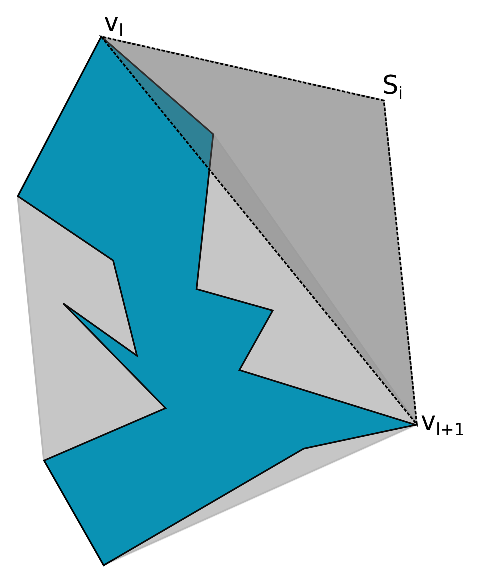
\includegraphics[width=0.38\textwidth]{img/steadyTriangle.eps}
      \end{center}
      \vspace{-20pt}
      \caption{Dreieckspunkttest}
      \vspace{-10pt}
      \label{fig:steadyTraingle}
    \end{wrapfigure}
    Der Test, ob ein Punkt in der Konvexen H"ulle liegt, dauerte
    nach dieser Optimierung immer noch im worst-case $\bigO(n)$, dass konnte
    aber auf $\bigO(1)$ verbessert werden, aufgrund folgender Eigenschaft:

    Man beachte, dass in jeder Iteration $\CH(P_{i}) \cap S_i = \emptyset$ gilt.
    Damit befindet sich jedes neue $s_i$ au"serhalb der Konvexen H"ulle des
    Polygons. Wenn ein $s_i$ gew"ahlt und die neuen Konvexe H"ulle konstruiert
    wurde, dann bilden in der neuen Konvexen H"ulle die Eckpunkte $v_l$,
    $v_{l+1}$ vor und nach $s_i$ mit $s_i$ ein Dreieck $\triangle(v_l, s_i,
    v_{l+1})$. Da jeder Punkt aus der Punktmenge $S_i$ au"serhalb der alten
    Konvexen H"ulle liegt und uns nur diejenigen Punkte aus $S_i$ interessieren,
    die innerhalb der neuen konvexen H"ulle liegen, reicht es die Anfrage auf
    den Schnitt der beiden konvexen H"ullen zu konzentrieren. Da das Dreieck
    $\triangle(v_l, s_i, v_{l+1})$ diesen Schnitt komplett beinhaltet, kann die
    Anfrage auf dieses Dreieck weiter begrenzt werden.

    Nach~\cite{held98polygons} existiert immer eine vom Punkt $s_i$ aus
    sichtbare Kante im Polygon $P_i$. N"ahrere Details zur Implementierung diese
    Abschnittes des Algorithmus ist in der Laufzeitanalyse beschrieben.

  \subsubsection{Laufzeit}

    Nach dem Paper ist die Laufzeit $\bigO(n^2)$. Im Paper kostet pro
    Schleifendurchlauf das Berechnen der sichtbaren Kanten von dem gew"ahlten
    Punkt $s_i$ $\bigO(n)$. Das finden des Punktes $s_i$ soll auch in $\bigO(n)$
    m"oglich sein, leider wurde nicht angegeben, wie man einen passenden Punkt
    $s_i$ in $\bigO(n)$ finden kann, der trotzdem zuf"allig ist.

    In unserer Implementierung braucht das Suchen nach $s_i$ im worst-case
    $\bigO(n^2)$, wenn in jeder Iteration nur ein Punkt rausgenommen wird. Der
    Test, ob ein Punkt in der erweiterten Konvexen H"ulle liegt, ist aufgrund
    der obigen Beobachtung in $\bigO(1)$ m"oglich (Punkt in Dreieck). Wenn in
    jedem Schritt ungef"ahr die H"alfte der Punkte eliminiert werden, dann
    kommen wir auf eine Laufzeit von $\bigO(n)$. Dies lies sich auch empirisch
    bei 100 Durchl"aufen mit je 1000 Punkten best"atigen. Durchschnittlich waren
    2 bis 3 Iterationen und in allen Durchl"aufen maximal 10 Iterationen
    notwendig, um $s_i$ zu finden. Bei gr"o"seren Punktmengen (2000, 3000, 4000)
    ergaben mit weniger Durchl"aufen ($10$ bis $20$) "ahnliche Ergebnisse
    (durchschnittlich 2 bis 3 Iterationen, maximal 12 Iterationen).
    Durchschnittlich dauerte das Suchen nach $s_i$ bei 1000 Punkten
    $0.100$\footnote{Messwerte auf einem Intel Atom N450 mit 1.66Ghz ermittelt}
    bis $0.180$ms und bei 2000 Punkte $0.150$ bis $0.200$ ms. Wie oben schon
    beschrieben, haben wir auf Optimierungen nach der Suche von $s_i$
    verzichtet, obwohl dies m"oglich ist.

    Das Suchen nach der sichtbaren Kante dauerte empirisch deutlich l"anger.
    Dies ist weiter nicht Verwunderlich, da wir eine einfache Implementierung
    f"ur das finden einer von $s_i$ sichtbaren Kante haben. Wir gehen jeden
    Eckpunkt des Polygons durch, bis zwei aufeinander folgende Eckpunkte $v_k,
    v_{k+1}$ von $s_i$ sichtbar sind. Daf"ur schneiden wir das Polygon mit der
    Strecke $\overline{s_i v_k}$. Das dauert bei uns $\bigO(n)$, womit insgesamt
    $\bigO(n^2)$ Zeit ben"otig wird, um die Kante zu finden. Durchschnittlich
    dauerte das Suchen nach der sichtbaren Kante bei 1000 Punkten $120$ bis
    $150$ ms und bei 2000 Punkten $233$ bis $343$ ms. Damit besitzt der
    Algorithmus hier Optimierungspotenzial.

    Somit braucht unsere Implementierung von \enquote{Steady Growth}
    $\bigO(n^3)$ Zeit.

  \subsubsection{Eigenschaften}

    Da \enquote{Steady Growth} von innen nach au"sen w"achst, sind in dem
    resultierenden Polygon viele Verzweigungen und Verwindungen. Mittelgro"se
    Punktmengen mit 1000 bis 2000 Punkten sind in vertretbarer Zeit generierbar.
    Und die Punkte des erzeugten Polygon sind in CCW angeordnet. Im Paper
    \cite{held98polygons} wird angemerkt, dass \enquote{Steady Growth} nicht
    jedes m"ogliche Polygon erzeugen kann.

\subsection{2-Opt Moves}

  \begin{figure}[h]
    \begin{center}
      
\includegraphics[width=0.3\textwidth]{img/2opt200.eps}
    \end{center}
    \caption{Polygon mit 200 Punkten (2-Opt Moves)}
    \label{fig:2opt200}
  \end{figure}

  \emph{2-Opt Moves} ist ein einfacher, randomisierter Algorithmus zur
  Erzeugung von simplen Polygonen, implementiert nach einer Beschreibung von
  Martin Held in~\cite{held98polygons}.    \subsubsection{Algorithmus}   Im
  ersten Schritt des Algorithmus werden die Punkte einer gegebenen Punktmenge
  zufällig zu einem komplexen Polygon verbunden, ähnlich der Vorgehensweise von
  \emph{Permute \& Reject}. Anschließend werden die Überschneidungen der Kanten
  des Polygons mit Hilfe eines sogenannten \enquote{2-opt move} repariert (s.
  Abbildung~\ref{fig:2optmove}), bis ein überschneidungsfreies Polygon
  entstanden ist.

  \begin{figure}[h]
    \begin{center}
      \subfigure[Vorher]{
        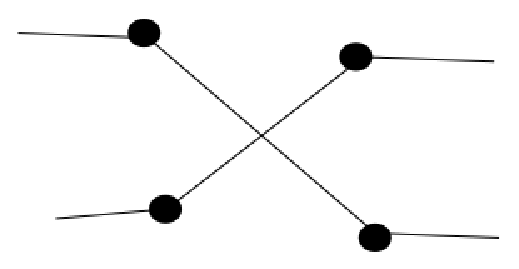
\includegraphics[width=0.4\textwidth]{img/2optbefore.eps}
        \label{fig:2optbefore}
      }
      \subfigure[Nachher]{
        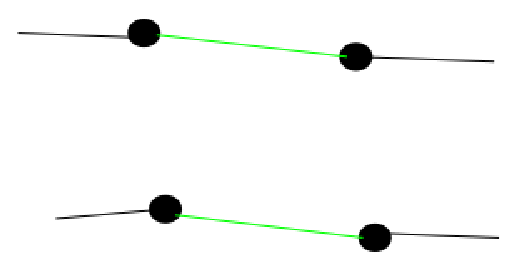
\includegraphics[width=0.4\textwidth]{img/2optafter.eps}
        \label{fig:2optafter}
      }
    \end{center}
    \caption{Beispiel eines 2-Opt Move}
    \label{fig:2optmove}
  \end{figure}

  \subsubsection{Eigenschaften}

    Laut Held wächst das theoretische Maximum der zur Entfernung aller Schnitte
    notwendigen 2-Opt moves kubisch mit der Anzahl der gegebenen Punkte, in der
    Praxis sei die Anzahl der durchgeführten 2-Opt moves jedoch eher quadratisch
    in Abhängigkeit von $n$. In Verbund mit der von uns implementierten, naiven
    Polygon-Schnitt-Suche (in $\bigO(n^2)$) erhalten wir ein theoretisches
    asymptotisches Wachstum der Laufzeit von $\bigO(n^4)$. Da die einzelnen
    Schritte des Algorithmus jedoch wenig rechenintensiv sind, eignet sich
    \emph{2-Opt Moves} durchaus zur Konstruktion simpler Polygone mit bis zu
    2000 Punkten. Die resultierenden Polygone wirken zudem sehr zufällig und
    weisen (im Gegensatz bspw. zu \emph{Steady Growth}) keinerlei vorherrschende
    \enquote{Kantenrichtung} auf.
    
\subsection{Velocity Virmani}

\begin{figure}[h]
\begin{center}

\includegraphics[width=0.3\textwidth]{img/virmani200.eps}
\end{center}
\caption{Polygon mit 200 Punkten (Velocity Virmani)}
\label{fig:virmani200}
\end{figure}

Der Algorithmus \enquote{Velocity Virmani} wurde am 25. Juli 1991 in dem Paper \enquote{Generating Random Polygons} von Joseph O'Rourke und Mandira Virmani veröffentlicht \cite{virmani91polygons}.\smallskip \\ 
Er beschreibt einen Algorithmus zur Generierung zufälliger simpler Polygone mittels Verschiebungen von Punkten. In dem genannten Paper wurde dem Algorithmus kein Name gegeben, deshalb haben wir uns die Freiheit genommen und werden in unserer Ausarbeitung mit dem Namen \enquote{Velocity Virmani} oder \enquote{Virmani} darauf verweisen.

Der Algorithmus besteht aus 3 Kernkomponenten:
\begin{enumerate}
	\item Die Generierung von einem regulären Polygon with n Punkten
	\item Zufällige Verschiebungen der Eckpunkte
	\item Die Überprüfung ob das Polygon noch simpel ist
\end{enumerate}

\subsubsection{Generierung des regulären Polygons}
Eingabeparameter: 
\begin{itemize}
	\item Anzahl der Punkte(n)
	\item Radius(r)
\end{itemize}
Ausgabe:
\begin{itemize} 
	\item Reguläres Polygon mit n Punkten
\end{itemize}
Hier wird ein reguläres Polygon generiert indem man auf einem Kreis n Punkte gleichmäßig verteilt und diese dann miteinander verbindet. Um zu berechnen wo jeder einzelne Punkt gesetzt wird muss vorher der Abstand zwischen jedem Punkt berechnet werden. Dazu nimmt man den vollen Kreisradius (PI*2) und teilt diesen durch die Anzahl der Punkte(n): $winkel = (PI * 2) / n$.\\ 
Das Ergebnis ist der Abstand, als Winkel, zwischen jedem einzelnen Punkt.
Mit dem Radius zusammen kann man dann die jeweiligen Koordinaten des regulären Polygons berechnen:\\
$x_i = r * cos(winkel * i)$\\
$y_i = r * sin(winkel * i)$

\subsubsection{Verschiebung}
Eingabeparameter: 
\begin{itemize}
	\item Boundaries(boundary)
	\item simples Polygon welches in den Boundaries ist(polygon)
	\item maximale Geschwindigkeit(maxvelocity)
	\item Anzahl der Durchläufe (iterations)
\end{itemize}
Ausgabe:
\begin{itemize}
	\item Zufälliges Polygon
\end{itemize}
In diesem Teil wird jeder Punkt zufällig verschoben, die maximale Distanz, die sich ein Punkt pro Achse bewegen kann, wird eingegrenzt durch den Eingabeparameter maxvelocity. Nach jeder Verschiebung von einem Punkt können folgende Zustände auftreten:
\begin{enumerate}
	\item Das Polygon ist simpel und in den Grenzen (Boundaries)
	\item Das Polygon ist simpel aber außerhalb der Grenzen
	\item Das Polygon ist nicht simpel aber innerhalb der Grenzen
	\item Das Polygon ist weder simpel noch in den Grenzen
\end{enumerate}
Sollte es vorkommen das der Zustand nicht Punkt 1 enspricht (simpel und in den Grenzen), so wird die Verschiebung rückgängig gemacht und für diesen Punkt im Polygon ändert sich nichts.
Dieser gesamte Prozess wird \enquote{iterations}-oft ausgeführt sodass es wirklich zufällig wird.

\begin{code}[caption={Pseudocode},mathescape=true]
for (int i=0; i < iterations; i++)
{
	foreach($p_i$ in polygon)
	{
		move_point_randomly($p_i$, maxvelocity);
		if(isSimple(polygon) && isInBound(polygon))
			continue;
		else
			revert_move_point_randomly($p_i$);
	}
}
\end{code}

\subsubsection{Überprüfen ob das Polygon simpel ist}
In dem Velocity Virmani wird nach jedem Punkt getestet ob das Polygon noch simpel ist. Dies kann bei einer trivialen Implementierung des Tests mit $n^3$ zu sehr hohen Laufzeiten führen.
Deshalb ist ein trivialer Test nach der Eigenschaft simpel nicht effizient.\smallskip \\ 
Die Lösung für dieses Problem besteht darin nur die angrenzenden Linien des verschobenen Punktes mit allen anderen Linien auf Überschneidungen zu überprüfen. Eine komplette Überprüfung auf Simplizität ist nicht nötig.
Der Algorithmus dafür wäre trivial und würde die Laufzeit für einen Test von $\bigO(n^3)$ auf $\bigO(n)$ sinken.

Vorraussetzung: Polygon muss vor der Verschiebung simpel sein
Eingabeparameter: Polygon, der verschobene Punkt(u)
Es werden die beiden zugehörigen Kanten von dem Punkt u genommen. Diese beiden Kanten werden mit den allen restlichen Kanten auf eine Schnittmenge überprüft. Sollte sich bei irgendeiner Kante eine Schnittmenge ergeben, so ist das Polygon nicht simpel und es muss nicht weiter getestet werden. Eine Ausnahme bilden jedoch die Endpunkte von den Kanten, jede Kante darf sich genau ein Endpunkt mit einer anderen Kante teilen.


\subsubsection{Eigenschaften}
\begin{itemize}
	\item Nichtdeterministisch\\
	Das Programm ist nichtdeterministisch da es für die Verschiebung von Punkten einen Zufallsgenerator nutzt. Somit kann man davon ausgehen das bei gleicher Eingabe von Parametern nicht immer die gleiche Ausgabe entsteht (für $maxvelocity > 0$)
	\item Komplexität: $\bigO(iterations*n^2)$\\
	Die Komplexität setzt sich zusammen aus der Anzahl der Iterationen, aus der Anzahl der Punkte durch welche iteriert wird um die Verschiebungen durchzuführen und nochmal durch die Anzahl der Punkte für den Test auf Simplizität. Somit ergibt sich eine Laufzeit von $\bigO(iterations*n*n) = \bigO(iterations*n^2)$
	\item Terminiert\\
	Der Algorithmus terminiert immer da die Anzahl der Schlaufendurchgänge begrenzt ist. Es gibt keinen Zustand im Algorithmus wo er verbleiben kann.
\end{itemize}

%TODO Überdenke diese Section und verkürze sie evtl.
%velocity <-> boundary box <-> radius <-> n
%velocity <-> radius
%space per point: boundary box <-> n
\subsubsection{Zufälligkeit der Polygone in Abhängigkeit von Parametern}
Der Algorithmus generiert zuverlässig zufällige Polygone bei der \enquote{richtigen} Eingabe von Parametern. Folgende Parameter haben Abhängigkeiten untereinander welches die Zufälligkeit des Polygons beeinflussen:\\
\textit{maxvelocity <-> boundary box <-> radius <-> n}

Die maximale Verschiebung die ein Punkt haben kann, kann nicht größer der Boundary Box sein. Deshalb ist es nicht effektiv diese höher zu setzen da es dazu führt das viele Bewegungen rückgängig gemacht werden.
Der Radius hat eine Abhängigkeit von der Boundary Box, da diese bestimmt wieviel Platz zum Wachsen, nach innen oder außen, vorhanden ist.\\
Die Anzahl der Punkte haben eine Abhängigkeit zu dem Radius und damit auch zu der maximalen Bewegungsgeschwindigkeit und der Boundary Box weil eine große Menge an Punkten den Raum den man sich teilt einschränkt.
\paragraph{Schlussfolgerung:}
Alle erwähnten Parameter haben eine Abhängigkeit bezüglich des Raumes die es sich teilen. Die Parameter sollten so gewählt sein das die Punkte genug Platz zum wachsen haben, sowie aber auch nicht so gewählt werden das sie beliebig wachsen können. Ein Mittelmaß an Kollisionen für eine effektive Generierung an Polygonen ist erwünscht.
Der einzige Parameter der keine Abhängigkeit zum Raum der Punkte hat, ist der Parameter iterations. Iterations bestimmt die Anzahl der Durchläufe von Bewegungen. Durch das hochsetzen dieses Parameters ist es möglich die Zufälligkeit eines Polygons zu erhöhen trotz schlecht gewählter Parameter. Jedoch ist dies nicht empfehlenswert da es die Laufzeit sehr stark erhöhen kann.  

%info Die sauberere schönere Erklärung auswählen
%\begin{itemize}
%	\item \\
	
%	\item maximale Geschwindigkeit <-> Boundary Box\\
%	Die maximale Geschwindigkeit die ein Punkt pro Durchlauf annehmen kann ist abhängig von der Boundary Box. Es ist zum Beispiel nicht effektiv bei einer Boundary Box von 500x500 eine maximale Geschwindigkeit von 1000 festzulegen, da diese nicht erreicht werden kann. Der Effekt dabei ist das die Wahrscheinlichkeit das ein Punkt am Ende sich nicht bewegt weil es out of Bound ist, oder kollidiert, sehr hoch wird. Dadurch wird die Zufälligkeit des Polygons beeinflusst.\\
%	Die maximale Geschwindigkeit zu klein zu setzen führt wiederrum dazu das man viele Iterationen braucht um mehr Weg bewältigen. Bei wenigen Iterationen würde somit das Polygon weniger zufällig sein.
%	\item n <-> Boundary Box <-> maximale Geschwindigkeit\\
%	Je größer die Anzahl der Punkte ist desto größer sollte die Boundary Box sein. Denn je mehr Punkte beisammen liegen, desto höher ist die Chance bei größeren Bewegungen das die Punkte \enquote{rejected} werden. Dies kann man Vorbeugen indem man die maximale Geschwindigkeit kleiner setzt. Jedoch sollte man auch hier Punkt 1 beachten.
%	\item Radius <-> Boundary Box\\
%	Das reguläre Polygon sollte so gesetzt werden das es mittig in der Boundary Box liegt. Idealerweise sollte die Entfernung von dem Polygon zur Boundary Box ungefähr dem Radius entsprechen.\\
%	Der Grund dafür liegt darin das wenn die Boundary Box zu klein ist, das viele Bewegungen der Punkte welche nach außen gehen \enquote{rejected} werden.
%	\item Radius <-> n\\
%	Hier ist es wichtig das man nicht zuviele Punkte so dicht zusammenpackt. Das Problem ist wie bei den oben genannten Punkten das sonst sich die Punkte nicht frei bewegen können.
%\end{itemize}

%TODO statt paragraph evtl. was anderes nutzen
%\paragraph{Fazit}
%Wie man sehen kann sind fast alle Parameter voneinander in gewisser Weise abhängig. Dies liegt daran das die folgenden Parameter jeweils den Raum der Punkte oder deren Bewegung bestimmen: n, boundary, maxvelocity, radius.\\
%Der einzige Parameter der keine Abhängigkeit zu den Punkten oder zu dem Raum hat ist der Parameter \enquote{iterations}. Dieser Parameter kann bei genug hoher Festlegung dazu führen das selbst sehr ungünstig gesetzte Parameter zu einem guten, zufälligen Ergebnis führen.\\
%Jedoch ist dies nicht empfehlenswert da Iterations einen starken Einfluss auf die Laufzeit hat und dies dazu führen kann das hohe Laufzeiten entstehen.

\subsection{Two Peasants}

  \begin{figure}[h]
    \begin{center}
      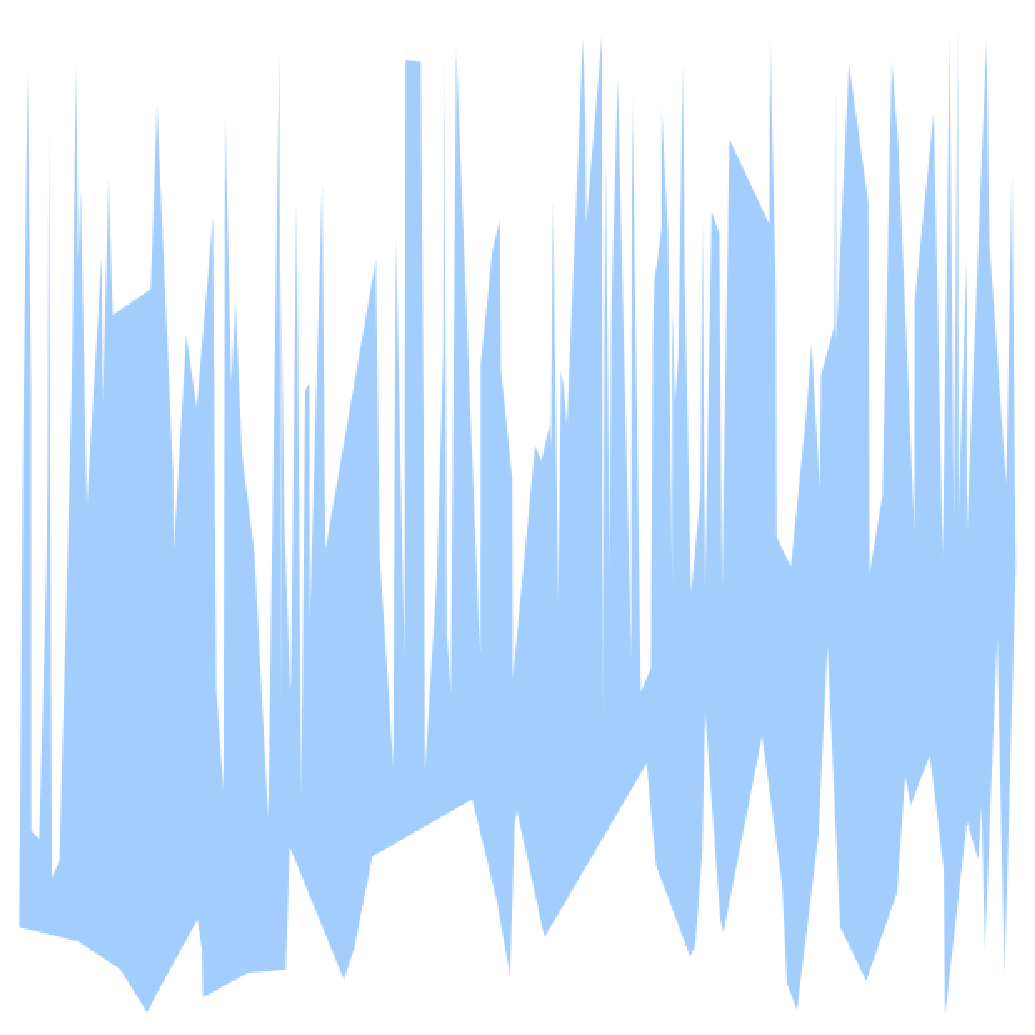
\includegraphics[width=0.3\textwidth]{img/twopeasants200.eps}
    \end{center}
    \caption{Polygon mit 200 Punkten (Two Peasants)}
    \label{fig:twopeasants200}
  \end{figure}

  \emph{Two Peasants} ist ein sehr einfacher Algorithmus ähnlich dem Algorithmus
  zur Erzeugung der konvexen Hülle einer Punktmenge, implementiert nach einer
  Beschreibung in~\cite{geometrylab}.

  \subsubsection{Algorithmus}

    Ausgehend von einer nach der $x$-Koordinate sortierten Punktmenge wird
    zunächst eine imaginäre Gerade zwischen den Extrempunkten gezogen.
    Oberhalb dieser Geraden werden anschließend die Punkte, die links der
    Geraden liegen, in Reihenfolge ihrer $x$-Koordinate verbunden.
    Anschließend werden die restlichen Punkte unterhalb der Geraden in
    umgekehrte Reihenfolge verbunden.

  \subsubsection{Eigenschaften}

  Der \emph{Two Peasants}-Algorithmus ermöglicht nicht die Erzeugung sämtlicher
  auf Grundlage einer Punktmenge denkbaren Polygone; er erzeugt im Gegenteil
  stets das selbe einfache Polygon. Die erzeugten Polygone lassen mit
  zunehmender Punktzahl deutlich die imaginäre Gerade zwischen den Extrempunkten
  erkennen. Oberhalb und unterhalb dieser Geraden entstehen zunehmend vertikale
  Strecken als Verbindung zwischen aufeinanderfolgenden Punkten der Punktmenge.
  Der Algorithmus ähnelt der natürlichen Vorgehensweise eines Menschen, der
  versucht aus einer gegebenen Punktmenge ein simples Polygon zu konstruieren
  (vgl.~\cite{geometrylab}). Die Laufzeit des Algorithmus wird dominiert von der
  Laufzeit des gewählten Sortieralgorithmus (bspw. im Normalfall $\bigO(n \log
  n)$), das Verbinden der sortierten Punkte zu einem Polygon erfolgt
  anschließend in linearer Zeit.

\subsection{Random Polygon Algorithm} % (fold)

\begin{figure}[h]
\begin{center}

\includegraphics[width=0.3\textwidth]{img/rpa200.eps}
\end{center}
\caption{Polygon mit 200 Punkten (Random Polygon Algorithm)}
\label{fig:virmani200}
\end{figure}

\label{sub:random_polygon_algorithm}

  Der \textit{Random Polygon Algorithm} (RPA) ist ein von Dailey und
  Whitfield in~\cite{dailey08rpa} beschriebener Algorithmus zur Erzeugung
  beliebiger Repräsentanten aus der Klasse aller einfachen Polygone.

  \subsubsection{Algorithmus} % (fold)
  \label{ssub:algorithmus}

    Der RPA arbeitet im Gegensatz zu den anderen hier aufgefürten
    Algorithmen nicht auf einer gegebenen Punktmenge. Stattdessen werden
    alle Punkte des erzeugten Polygons zur laufzeit berechnet und
    eingefügt. Zur initialisierung werden zunächst drei beliebige Punkte
    innerhalb der Boundingbox gewählt. Anschliessend werden für ein n-gon
    die folgenden Schritte (n-3)-mal ausgeführt:

    \begin{itemize}
      \item Wähle eine zufällige Kante $V_aV_b$ des Polygons.
      \item Bestimme die von dieser Kante sichtbare Region.
      \item Wähle einen zufälligen Punkt $V_c$ innerhalb der 
            erzeugten sichtbaren Region und füge diesn in das 
            Polygon ein. Ersetze die Kante $V_aV_b$ durch die Kanten 
            $V_aV_c$ und $V_cV_b$.
    \end{itemize}

    Zur Bestimmung der sichtbaren Region wird als erstes die von der Kante AB
    sichtbare Region innerhalb des Polygons ermittelt. Anschliessend wird die
    von AB sichtbare Region ausserhalb des Polygons und innerhalb der
    Boundingbox bestimmt und mit der inneren verbunden. Zur Erzeugung des
    Punktes X wird die erhaltene Gesamtregion trianguliert und aus der
    erhaltenen Menge von Dreiecken eins gewichtet nach der Größe zufällig
    gewählt. Innerhalb dieses Dreiecks wird nun ein Punkt zufällig gewält und
    als Punkt X in das Polygon eingefügt. Für eine detailierte Beschreibung
    des Algorithmus siehe~\cite{dailey08rpa}.
  
  % subsubsection algorithmus (end)

  \subsubsection{Eigenschaften \& Implementierungsdetails} % (fold)
  \label{ssub:eigenschaften}

    Um den inneren und äußeren Teil der von $V_aV_b$ sichtbaren Region
    aufzubauen ist es nötig zu bestimmen ob ein Punkt von $V_a$ und von $V_b$
    aus sichtbar sind. Zudem werden sichtbare Punkte in von innen sichtbare
    (d.h. die Sichtlinie befindet sich gänzlich innerhalb des Polygons) und
    von aussen sichtbare (d.h. die Sichtlinie befindet sich gänzlich
    ausserhalb des Polygons, jedoch innerhalb der Boundingbox) unterteilt.
    In~\cite{dailey08rpa} wird hierzu ein einfacher Test auf Schnittpunkte mit
    der Kante $V_aV_b$ vorgeschlagen, jedoch nicht beschrieben, mit welcher
    weiteren Kante $V_aV_b$ geschnitten wird. Für einen Punkt $V_x$ ist es
    jedoch mit einem Sichtbarkeitstest und zwei Winkeltest möglich zu
    bestimmen, ob der Weg auf dem Polygon von $V_a$ bzw. $V_b$ zu $V_x$ links
    oder rechts der Sichtlinie von $V_a$ bzw. $V_b$ zu $V_x$ liegt.

    Die von Dailey und Whitfield in~\cite{dailey08rpa} abgeschätzte worst-case
    Laufzeit des RPA beträgt $\bigO(n^3)$. Hierbei gehen sie von einer
    Triangulierung in $\bigO(n \log n)$ aus. Der von uns verwendete Ear
    Clipping Algorithmus erreicht jedoch nur eine Laufzeit von $\bigO(n^2)$,
    so dass die worst-case Laufzeit des RPA insgesamt auf $\bigO(n^4)$ steigt.
    Mit einem schnelleren, jedoch gleichzeitig wesentlich komplexeren
    Triangulierungsalgorithmus wie dem von Seidel~\cite{seidel91asimple} wäre
    die von Dailey und Whitfiel abgeschätzte Laufzeit auch mit der
    vorliegenden Implementierung des RPA zu erreichen.

    Von den von uns implementierten Algorithmen ist der RPA der einzige,
    welcher Repräsentanten aus der Klasse aller einfachen Polygone erzeugt.
    Der von Dailey und Whitfield hierzu geführete Beweis ist in
    ~\cite{dailey08rpa} zu finden.

  % subsubsection eigenschaften (end)

% subsection random_polygon_algorithm (end)
\section{Shortest Path}
	%abbildung einfügen

  Unsere Implementierung des Shortest-Path Algorithmus basiert auf dem Paper
  \enquote{Constant-Work-Space Algorithms For Geometric Problems} Asano et.
  al.~\cite{asano11shortestpath}.

  \subsection{Algorithmus}

    Der Algorithmus benutzt ein Tripel aus drei Punkten ($p$,$q_1$,$q_2$) um
    durch das Polygon zu navigieren. Es gilt, dass der Punkt $p$ ein Punkt des
    Shortest-Path ist und das Polygon hinter $q_1$, $q_2$ den Zielpunkt ($t$)
    enthält. Um dies zu erreichen wird zu Beginn das Polygon in Trapeze
    unterteilt. Vom Startpunkt aus wird ein Dreieck zu jeweils zwei
    benachbarten Eckpunkten des Trapezes aufgespannt und geprüft, ob das
    dahinter liegende Polygon den Zielpunkt enthält. Der triviale Fall, in dem
    sich der Zielpunkt im gleichen Trapez befindet wie der Startpunkt wird zu
    Beginn überprüft. Ausgehend von dem Trapez in dem der Startpunkt liegt
    wird das Polygon so reduziert, dass sich der Zielpunkt immer noch
    innerhalb des Polygons befindet. Um den nächsten Punkt des Shortest-Path
    zu finden wird die Krümmung von $p$,$q_1$,\texttt{succ}($q_1$) bzw
    $p$,$q_2$,\texttt{pred}($q_2$) betrachtet, wobei \texttt{pred} und
    \texttt{succ} jeweils den Vorgänger und Nachfolger des jeweiligen Punktes
    in der Polygonkette bezeichnen.

  \subsection{Implementierung}

    Bei der Implementierung konnten wir uns größten Teils an die Vorgaben des
    Paper halten. Allerdings stellte sich das Unterteilen des Polygons in
    Trapeze als schwieriger heraus, als zunächst angenommen. Schließlich
    entschieden wir uns, auf die Unterteilung zu verzichten und stattdessen
    einen etwas einfacheren Ansatz zu verwenden. Die Initialisierung des
    Starttripel funktioniert folgendermaßen:

    \begin{enumerate}
      \item Finde alle Eckpunkte des Polygons, die direkt vom Startpunkt aus
            sichtbar sind.
      \item Erzeuge von je zwei Eckpunkten und dem Startpunkt ein Subpolygon
            und überprüfe ob $t$ darin liegt.
      \item Falls $t$ in dem Polygon liegt ist die Startkonfiguration gefunden,
            andernfalls untersuche die nächsten zwei Punkte.
    \end{enumerate}

    Unter anderem aus diesem Grund haben wir uns vorwiegend darauf konzentriert, eine
    funktionierende Implementierung umzusetzen. Laufzeit und Speicherverbrauch
    sind daher nicht optimal und es gibt sehr viel Optimierungspotential. Daher konnten 
    wir auch nicht dem ursprünglichen Anspruch von konstantem Speicherverbauch gerecht werden.

\newpage
  \subsection{Laufzeit}

  Die Laufzeit der Implementierung lässt sich mit $O(5n^2)$ abschätzen:

  \begin{itemize}
  \item Initialisierung des Tripel: $O(2n^2)$
        \begin{itemize}
        \item Berechnung der vom Startpunkt aus sichtbaren Punkte: $O(n^2)$\\
        Um zu überprüfen, welche Punkte vom Startpunkt aus sichtbar sind
        werden alle Streckenabschnitte jeweils vom Startpunkt bis zu einem
        Eckpunkt des Polygons mit jeder Kante des Polygons geschnitten.
        \item Überprüfung der Initialisierung des Tripel: $O(n^2)$\\
        Für jeden Tupel von sichtbaren Punkten wird das Polygon reduziert
        (weitere Erklärungen unten) und anschließend geprüft ob $t$ darin liegt.
        \end{itemize}
  \item Nach der Initialisierung wird solange der Zielpunkt nicht sichtbar ist
        der nächste Schritt berechnet: $n \cdot O(3n) = O(3n^2)$
        \begin{itemize}
        \item Überprüfung, ob der Zielpunkt sichtbar ist: $O(n)$\\
        Die Strecke ($p,t$) wird mit jeder Kante des Polygons geschnitten wird.
        \item Berechnung des nächsten Schrittes: $O(2n)$
          \begin{itemize}
          \item Zuerst wird das Polygon reduziert: $O(n)$
          \item Die Krümmung der nächsten Kante des Polygons berechenen: $O(1)$
          \item Der Schnittpunkt zwischen dem Stahl (abhängig von der vorher
          berechneten Krümmung) und Polygon wird berechnet: $O(n)$
          \item Das neue Tripel wird zurückgegeben: $O(1)$
          \end{itemize}
        \end{itemize}
  \end{itemize}

  Weitere Erklärungen:

  \begin{itemize}
  \item Reduzierung des Polygons: $O(n)$\\
        Die Polygon Punktliste wird so umgestellt, dass sich ($q_1$) am Anfang der
        Liste befindet ($O(1)$). Es werden schrittweise Punkte hinzugefügt, bis
        der Punkt ($q_2$) gefunden wird ($O(n)$). Das Polygon kann jetzt mit dem
        Hinzufügen von ($q_2$) und ($p$) geschlossen werden.
  \item Schnitt von Polygon und Strahl: $O(n)$\\
        Der Strahl wird mit jeder Kante des Polygons geschnitten
  \end{itemize}

  \subsection{Speicherverbrauch}

  Der Speicherverbrauch lässt sich mit $O(n^2)$ abschätzen. Dies lässt sich zum
  einen dadruch erklären, dass wir den Algorithmus in Java implementiert haben
  und so praktisch keine Einfluss auf die Speicherverwaltung nehmen können. Zum
  anderen haben wir, um Code-Duplizierung zu vermeiden, die meisten Funktionen
  ausgelagert um sie auch in anderen Methoden benutzten zu können. Dabei haben wir
  meist keine Speicherbereiche mit übergeben, welches natürlich einen stark
  erhöhten Speicherverbauch mit sich bringt. Mit ein wenig Optimierung sollte man
  aber auch unserse Implementierung mit einem Speicherverbrauch von $O(n)$
  realisieren können. Wenn man den originalen konstanten Speicherverbrauch
  erreichen möchte sollte man die Programmiersprache C verwenden.







\section{Manual}
\label{sec:manual}
\subsection{Dependencies \& Compilation}
\subsection{Graphische Oberfläche}
\subsection{Kommandozeile}

\cleardoublepage
\phantomsection

% Bibliography
\addcontentsline{toc}{section}{Literatur}
\bibliographystyle{alpha}
\bibliography{report}

\end{document}
